%!TEX root=../main.tex
\section{Method} % (fold)
\label{sec:method}

The primary thing to consider to convert the shots charts into functional datasets. To do so, we employed a 2-dimensional kernel density estimation for both the attempted and made shots, utilizing Silverman's rule \cite{silvermanDensityEstimationStatistics1986} for the estimation of the bandwith. The density estimation is conducted on a regularly spaced grid consisting of $201 \times 201$ points. We obtain observations of bivariate functional data, where both features are defined on a two-dimensional rectangular domain, and observed on an equidistant grid of size $201 \times 201$. Figure~\ref{fig:examples_shooting_density} presents the density estimation of the same five players than for the shots charts in Figure~\ref{fig:examples_shooting_charts}. 

\textcolor{red}{The method can be summarized with these steps:
\begin{enumerate}
    \item 2D Kernel density estimation
    \item MFPCA
    \item Clustering
\end{enumerate}}


\textcolor{red}{We estimate the functional principal components using the \texttt{Gram}, \texttt{(Tensor) PCA} and \texttt{2D/1D B-Splines} methods. For the \texttt{Gram} method, we directly use the estimated densities to estimate the eigencomponents. For the \texttt{(Tensor) PCA} method, the estimation of the multivariate eigenimages is based on the univariate estimation of $30$ univariate eigenimages. The estimation of the (univariate) eigenimages is performed with the FCP-TPA where the smoothing parameters are chosen via cross-validation in $[10^{-5}, 10^5]$. For the \texttt{2D/1D B-splines} method, the two components are expanded in tensor products of $13 \times 13$ B-splines. We do not add a smoothing penalty in that case, as the smoothing step is performed in the kernel density estimation.}

\textcolor{red}{Clustering of the scores in the FPCA basis. I would probably use $k$-means with $k = 5$, it makes sense to have $k = 5$ because there are $5$ players of the court.}


\begin{figure}
    \centering
    
\includegraphics[scale=0.35]{figures/curry_density.eps}
    
\includegraphics[scale=0.35]{figures/tatum_density.eps}
    
\includegraphics[scale=0.35]{figures/james_density.eps}
    
\includegraphics[scale=0.35]{figures/embiid_density.eps}
    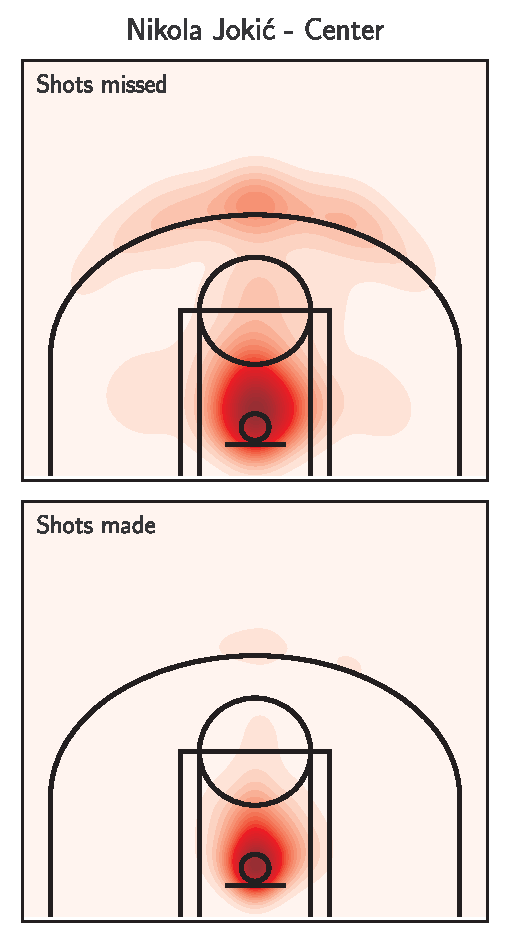
\includegraphics[scale=0.35]{figures/jokic_density.eps}
    \\
    
\includegraphics[scale=0.35]{figures/colorbar.eps}
    \caption{Shots charts density for five selected NBA players. Note that the densities have been individually normalized between $0$ and $1$.}
    \label{fig:examples_shooting_density}
\end{figure}


% section method (end)